% !TeX program = xelatex
\ifdefined\BookMaster\else
\documentclass[11pt,oneside]{article}
% !TeX program = xelatex
\usepackage[b5paper,left=22mm,right=22mm,top=20mm,bottom=22mm,footskip=11mm]{geometry}
\usepackage{fontspec}
\setmainfont{TeX Gyre Termes}
\setsansfont{TeX Gyre Heros}
\usepackage{amsmath,amssymb,mathtools,amsthm}
\renewcommand{\cdots}{\mathinner{\cdotp\cdotp\cdotp}}
\usepackage{graphicx,adjustbox,array,booktabs,longtable,multirow,enumitem,changepage,needspace}
\usepackage[table]{xcolor}
\usepackage{fancyhdr}
\raggedbottom
\interfootnotelinepenalty=10000
\newcommand{\BookFootnote}[2]{\begingroup\renewcommand{\thefootnote}{\fnsymbol{footnote}}\footnote[#1]{#2}\endgroup}
\newcommand{\BookFootnoteMark}[1]{\begingroup\renewcommand{\thefootnote}{\fnsymbol{footnote}}\footnotemark[#1]\endgroup}
\newcommand{\BookFootnoteText}[2]{\begingroup\renewcommand{\thefootnote}{\fnsymbol{footnote}}\footnotetext[#1]{#2}\endgroup}
\newenvironment{BookFloat}[1]{\par\addvspace{.6\baselineskip}\noindent\def\BookFloatID{#1}\begin{minipage}{\linewidth}\phantomsection\label{bookfloat:#1:start}}{\phantomsection\label{bookfloat:\BookFloatID:end}\end{minipage}\par\addvspace{.6\baselineskip}}

\usepackage[unicode,hidelinks]{hyperref}
\pagestyle{fancy}
\fancyhf{}
\newcommand{\BookFooter}{}
\fancyfoot[L]{\parbox[b]{\dimexpr\textwidth-15mm}{\footnotesize\BookFooter}}
\fancyfoot[R]{\footnotesize\thepage}
\renewcommand{\headrulewidth}{0pt}
\renewcommand{\footrulewidth}{0pt}
\setlength{\parindent}{0pt}
\setlength{\parskip}{0.2em}
\setlength{\emergencystretch}{3em}
\setlist{nosep,leftmargin=1.7em,labelsep=.65em}
\newif\ifBookNarrative
\BookNarrativetrue
\newenvironment{BookBody}{\setlength{\parindent}{0pt}}{}
\newcommand{\BookStatement}[1]{\par\addvspace{.6\baselineskip}\noindent #1\enspace\ignorespaces}
\newcommand{\BookLabel}[1]{\par\addvspace{.6\baselineskip}\needspace{3\baselineskip}\noindent\textbf{#1}\quad\ignorespaces}
\newcommand{\BookHeading}[1]{\par\addvspace{\baselineskip}\needspace{4\baselineskip}\noindent{\large\bfseries #1}\par\medskip}
\newcommand{\BookSubheading}[1]{\par\addvspace{.7\baselineskip}\needspace{3\baselineskip}\noindent{\bfseries #1}\par\smallskip}
\newcommand{\BookTextHeading}[1]{\par\addvspace{.7\baselineskip}\needspace{3\baselineskip}\noindent #1\par\smallskip}
\newcommand{\BookSectionTitle}[2]{\par\addvspace{1.2\baselineskip}\needspace{5\baselineskip}\noindent\colorbox{gray!25}{\sffamily\bfseries\small SECTION #1}\quad{\large\bfseries #2}\par\medskip}
\newcommand{\BookExerciseTitle}[1]{\par\addvspace{\baselineskip}\needspace{4\baselineskip}\noindent{\color{gray}\rule{1.5mm}{1.5mm}}\enspace{\large\bfseries Exercises #1}\par\medskip}
\newcommand{\BookBullet}[1]{\begin{list}{\textbullet}{\setlength{\leftmargin}{1.7em}\setlength{\labelwidth}{1em}\setlength{\labelsep}{.7em}\setlength{\topsep}{0pt}\setlength{\parsep}{0pt}\setlength{\itemsep}{0pt}}\item #1\end{list}}
\newcommand{\BookExercise}[2]{\begin{list}{\textbf{#1}}{\setlength{\leftmargin}{2.2em}\setlength{\labelwidth}{1.5em}\setlength{\labelsep}{.7em}\setlength{\topsep}{.15em}\setlength{\parsep}{0pt}\setlength{\itemsep}{0pt}}\item #2\end{list}}
\newcommand{\BookEnd}[1]{\unskip\nobreak\hfill\ensuremath{#1}}
\newcommand{\BookSource}[2]{\phantomsection\label{sourcepage:#1}} % Source-page anchors, retained through reflow.
\usepackage{multicol}
\usepackage{tikz}
\newcommand{\BookPartEntry}[2]{\par\noindent\makebox[17mm][l]{\bfseries Section #1}#2\par}
\newcommand{\BookPartTitle}[3]{\par\bigskip\noindent\begin{tikzpicture}\node[anchor=north west,inner sep=0pt,outer sep=0pt] (bookpart) at (0,0) {\begin{minipage}{\dimexpr\linewidth-.5pt}\hspace*{26mm}\begin{minipage}[t]{\dimexpr\linewidth-26mm}\begin{adjustbox}{max width=\linewidth}{\fontsize{20}{24}\selectfont\bfseries #2}\end{adjustbox}\par\vspace{6mm}\hrule\vspace{6mm}{\sffamily\footnotesize\setlength{\parskip}{.3em}#3}\vspace{3mm}\end{minipage}\end{minipage}};\path[shade,top color=gray!60,bottom color=white] (0,0) rectangle ([xshift=24mm]bookpart.south west);\node[anchor=north,font=\sffamily\bfseries\small] at (12mm,-2mm) {PART};\node[anchor=north,font=\sffamily\bfseries\Huge] at (12mm,-7mm) {#1};\end{tikzpicture}\par\bigskip}
\newsavebox{\BookMathBox}
\makeatletter
\newcommand{\BookInline}[1]{\leavevmode\hskip0pt\relax\begingroup\in@{\begin}{#1}\ifin@\sbox{\BookMathBox}{\(#1\)}\ifdim\wd\BookMathBox>\dimexpr\linewidth-1em\relax\resizebox{\dimexpr\linewidth-1em\relax}{!}{\usebox{\BookMathBox}}\else\(#1\)\fi\else\in@{\left}{#1}\ifin@\sbox{\BookMathBox}{\(#1\)}\ifdim\wd\BookMathBox>\dimexpr\linewidth-1em\relax\resizebox{\dimexpr\linewidth-1em\relax}{!}{\usebox{\BookMathBox}}\else\(#1\)\fi\else\(#1\)\fi\fi\endgroup\hskip0pt\relax}
\makeatother
\DeclareMathOperator{\Aut}{Aut}
\DeclareMathOperator{\End}{End}
\DeclareMathOperator{\Hom}{Hom}
\DeclareMathOperator{\GF}{GF}
\DeclareMathOperator{\irr}{irr}
\DeclareMathOperator{\lt}{lt}
\DeclareMathOperator{\lp}{lp}
\providecommand{\textcircled}[1]{\textnormal{(#1)}}

\begin{document}
\fi
\renewcommand{\BookFooter}{Section 43 Introduction to Galois Theory}
\pdfbookmark[0]{Section 43 Introduction to Galois Theory}{43_introduction_to_galois_theory}
\ifdefined\BookMaster\else\setcounter{page}{341}\fi
% Source PDF page 358; original printed page 341
\BookSource{358}{341}
\BookPartTitle{IX}{Galois Theory}{\BookPartEntry{43}{Introduction to Galois Theory}
\BookPartEntry{44}{Splitting Fields}
\BookPartEntry{45}{Separable Extensions}
\BookPartEntry{46}{Galois Theory}
\BookPartEntry{47}{Illustrations of Galois Theory}
\BookPartEntry{48}{Cyclotomic Extensions}
\BookPartEntry{49}{Insolvability of the Quintic}}

\BookNarrativetrue

\begin{BookBody}

\BookSectionTitle{43}{Introduction to Galois Theory}

\BookTextHeading{\textbf{An Example}  }

\noindent We learned in high school that the quadratic formula provides zeros for polynomials of degree two. There are similar formulas for solutions to polynomials of degree three and four. These solutions all involve addition, subtraction, multiplication, division, and taking radicals.\textbf{ Galois theory}, which provides an interesting connection between group theory and field theory, can be used to show that it is futile to seek a similar formula for polynomials of degree five or greater. Our main goal for the remainder of the book is to provide a proof of this fact.

\BookLabel{43.1 Definition} Let \BookInline{E} be a field. An\textbf{ automorphism} of \BookInline{E} is a isomorphism of \BookInline{E} onto itself. \BookEnd{\blacksquare}

\BookLabel{43.2 Theorem} The set of automorphisms of a field \BookInline{E} is a group under function composition.

\BookLabel{\textit{Proof}} The proof is Exercise 29. \BookEnd{\blacklozenge}

\BookLabel{43.3 Example} A field isomorphism \BookInline{\phi:E\to K} maps \BookInline{1\in E} to \BookInline{1\in K} and, it maps \BookInline{0\in E} to \BookInline{0\in K.} Therefore, for any automorphism \BookInline{\phi } of \BookInline{\mathbb{Q},\allowbreak \phi (1)= 1} and \BookInline{\phi (0)= 0.} It follows by induction that \BookInline{\phi (n)= n} for any natural number \BookInline{n.} Since \BookInline{\phi (- x)= - \phi (x),\allowbreak } for any integer \BookInline{n,\allowbreak } \BookInline{\phi (n)= n.} Every rational number is a ratio of integers, so \BookInline{\phi (r)= r} for every rational number \BookInline{r.} Therefore the only automorphism of \BookInline{\mathbb{Q}} is the identity map\BookInline{.}\BookEnd{\blacktriangle}

\BookLabel{43.4 Example} Let \BookInline{K= \mathbb{Q}(\sqrt{2},\allowbreak \sqrt{3}).} From Example 40.9, the degree of the extension \BookInline{K} over \BookInline{\mathbb{Q}} is 4 and a basis for the vector space \BookInline{K} over the field \BookInline{\mathbb{Q}} is \BookInline{\{1,\allowbreak \sqrt{2},\allowbreak \sqrt{3},\allowbreak \sqrt{6}\}.} Thus \BookInline{K= \{a+ } \BookInline{b\sqrt{2}+ c\sqrt{3}+ d\sqrt{6}|a,\allowbreak b,\allowbreak c,\allowbreak d\in \mathbb{Q}\}.} We determine the automorphisms of \BookInline{K.}

Let \BookInline{\phi } be any automorphism of \BookInline{K.} Since \BookInline{\phi (1)= 1,\allowbreak \phi } maps every rational number to itself as shown in the previous example. Since \BookInline{\phi } is a field automorphism\BookInline{,\allowbreak \phi (\sqrt{2^{2}}- 2)= } \BookInline{\phi (0)= 0.} But \BookInline{\phi(\sqrt{2}^{2}-2)=\phi(\sqrt{2})^{2}-2} Thus \BookInline{\phi (\sqrt{2})} is a zero of the polynomial \BookInline{x^{2}- } 2, which means that \BookInline{\phi (\sqrt{2})} is either \BookInline{\sqrt{2}} or \BookInline{- \sqrt{2}.} Similarly\BookInline{,\allowbreak \phi (\sqrt{3})= \pm \sqrt{3}.} Given any \BookInline{a,\allowbreak b,\allowbreak c,\allowbreak d\in \mathbb{Q},\allowbreak } if

\begin{center}\begin{adjustbox}{max width=\linewidth}\BookInline{\displaystyle \alpha = a+ b\sqrt{2}+ c\sqrt{3}+ d\sqrt{6}\in K,\allowbreak }\end{adjustbox}\end{center}

\end{BookBody}

% Source PDF page 359; original printed page 342
\BookSource{359}{342}
\BookNarrativetrue

\begin{BookBody}

\noindent then

\begin{center}\begin{adjustbox}{max width=\linewidth}\BookInline{\displaystyle \phi (\alpha )= a+ b\phi (\sqrt{2})+ c\phi (\sqrt{3})+ d\phi (\sqrt{2})\phi (\sqrt{3}).}\end{adjustbox}\end{center}

Once \BookInline{\phi (\sqrt{2})} and \BookInline{\phi (\sqrt{3})} are specified, there is at most one automorphism meeting these specifications. We have at most four automorphisms of \BookInline{K} given by Table 43.5.

\begin{BookFloat}{43_introduction_to_galois_theory-p359-3}
\begin{center}\small\textbf{43.5 Table}\end{center}
\begin{center}\begin{adjustbox}{max width=\linewidth}
\renewcommand{\arraystretch}{1.3}\setlength{\tabcolsep}{4pt}
\begin{tabular}{c|c|c|c}
 & $\phi(\sqrt2)$ & $\phi(\sqrt3)$ & $\phi(a+b\sqrt2+c\sqrt3+d\sqrt6)$\\\hline
$\iota$ & $\sqrt2$ & $\sqrt3$ & $a+b\sqrt2+c\sqrt3+d\sqrt6$\\
$\sigma$ & $-\sqrt2$ & $\sqrt3$ & $a-b\sqrt2+c\sqrt3-d\sqrt6$\\
$\tau$ & $\sqrt2$ & $-\sqrt3$ & $a+b\sqrt2-c\sqrt3-d\sqrt6$\\
$\gamma$ & $-\sqrt2$ & $-\sqrt3$ & $a-b\sqrt2-c\sqrt3+d\sqrt6$
\end{tabular}\end{adjustbox}\end{center}
\end{BookFloat}

It is tedious, but not difficult, to check that each of these maps is a field automorphism. By Theorem \BookInline{43.2,\allowbreak G= \{\iota,\allowbreak \sigma,\allowbreak \tau,\allowbreak \gamma \}} forms a group under function composition. Every group with exactly four elements is isomorphic with the Klein 4-group or the cyclic group of order four. Each element of \BookInline{G} has order one or two, so \BookInline{G} is isomorphic with the Klein 4-group\BookInline{.}\BookEnd{\blacktriangle}

\BookLabel{43.6 Definition} If \BookInline{E} and \BookInline{K} are both field extensions of a field \BookInline{F} and \BookInline{\sigma:E\to K} is a field isomorphism, then an element \BookInline{\alpha \in E} is\textbf{ fixed by} \BookInline{\sigma } if \BookInline{\sigma (\alpha )= \alpha.} An element \BookInline{\alpha \in E} is\textbf{ fixed by} a collection of isomorphisms if \BookInline{\alpha } is fixed by every isomorphism in the collection. A subset \BookInline{L} of \BookInline{E} is\textbf{ fixed by} a collection of isomorphisms if every \BookInline{\alpha \in L} is fixed by the collection. Often we write\textbf{ remains fixed} instead of simply fixed\BookInline{.}\BookEnd{\blacksquare}

The discussion in Example 43.3 shows that for any field extensions \BookInline{E} and \BookInline{K} of \BookInline{\mathbb{Q}} and isomorphism \BookInline{\sigma:E\to K,\allowbreak \mathbb{Q}} remains fixed by \BookInline{\sigma.}

\BookLabel{43.7 Example} We find the elements fixed by each of the four automorphisms of \BookInline{G} in Example 43.4. From Table 43.5 we see that each element fixes a subfield of \BookInline{\mathbb{Q}(\sqrt{2},\allowbreak \sqrt{3}),\allowbreak } and from this we can determine the field fixed by each subgroup of \BookInline{G.}

\BookBullet{Each element \BookInline{K} is fixed by \BookInline{\iota.} In other words\BookInline{,\allowbreak K} remains fixed by the trivial subgroup \BookInline{\{\iota \}.}}

\BookBullet{Each element of \BookInline{\{a+ c\sqrt{3}\mid a,\allowbreak c\in \mathbb{Q}\}= \mathbb{Q}(\sqrt{3})} is fixed by \BookInline{\sigma.} This implies that \BookInline{\mathbb{Q}(\sqrt{3})} remains fixed by the subgroup \BookInline{\langle \sigma \rangle \leq G.}}

\BookBullet{Each element of \BookInline{\{a+ b\sqrt{2}\mid a,\allowbreak b\in \mathbb{Q}\}= \mathbb{Q}(\sqrt{2})} is fixed by \BookInline{\tau.} So \BookInline{\mathbb{Q}(\sqrt{2})} remains fixed by the subgroup \BookInline{\langle \tau \rangle.}}

\BookBullet{Each element of \BookInline{\{a+ d\sqrt{6}\mid a,\allowbreak d\in \mathbb{Q}\}= \mathbb{Q}(\sqrt{6})} is fixed by \BookInline{\gamma.} Therefore\BookInline{,\allowbreak \mathbb{Q}(\sqrt{6})} remains fixed by the subgroup \BookInline{\langle \gamma \rangle.}}

\BookBullet{The only elements that remain fixed by \BookInline{G} are the elements of \BookInline{\mathbb{Q}.}}

Exercise 30 shows the five fields \BookInline{\mathbb{Q},\allowbreak \mathbb{Q}(\sqrt{2}),\allowbreak \mathbb{Q}(\sqrt{3}),\allowbreak \mathbb{Q}(\sqrt{6}),\allowbreak } and \BookInline{\mathbb{Q}(\sqrt{2},\allowbreak \sqrt{3}),\allowbreak } are the only subfields of \BookInline{K.} Furthermore, from group theory we know that \BookInline{G,\allowbreak \langle \sigma \rangle,\allowbreak \langle \tau \rangle,\allowbreak \langle \gamma \rangle,\allowbreak } and \BookInline{\{\iota \}} are the only subgroups of \BookInline{G.} We have established a one-to-one correspondence between the subfields of \BookInline{K} containing \BookInline{\mathbb{Q},\allowbreak } and the subgroups of the automorphism group of \BookInline{K} that fix elements of \BookInline{\mathbb{Q}.} Figure 43.8 shows the subfield diagram for \BookInline{K} and the subgroup diagram for \BookInline{G.} Notice that relabeling the fields by their corresponding subgroups gives the subgroup diagram, except that it is inverted. The reason that the diagrams are flipped is that if \BookInline{H_{1}\leq H_{2}} are both subgroups of the automorphism group of \BookInline{K,\allowbreak } then every element of \BookInline{K} fixed by all the automorphisms in \BookInline{H_{2}} is also fixed by all the elements of \BookInline{H_{1}.} So the set that remains fixed by \BookInline{H_{2}} is a subset of the set that remains fixed by \BookInline{H_{1}.}\BookEnd{\blacktriangle}

\end{BookBody}

% Source PDF page 360; original printed page 343
\BookSource{360}{343}
\BookNarrativetrue

\begin{BookBody}

\begin{BookFloat}{43_introduction_to_galois_theory-p360-0}
\begin{center}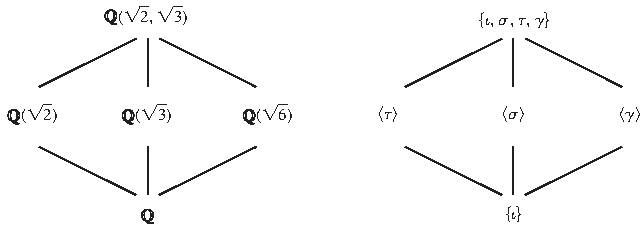
\includegraphics[width=0.882\linewidth,height=.8\textheight,keepaspectratio]{assets/p360_05.pdf}\end{center}
\begin{center}\small\textbf{43.8 Figure}\end{center}
\end{BookFloat}

The fact that the subfield diagram and the subgroup diagram correspond by associating a subfield of \BookInline{K} with a subgroup of \BookInline{G} is no accident. In fact, this is the heart of Galois theory. Before we can give precise statements of the Galois theorems, we need a few definitions and some background lemmas and theorems. It is advisable to have Examples 43.4 and 43.7 well in mind when reading the next few sections.

\BookTextHeading{\textbf{Subfields and Subgroups}  }

\noindent We now investigate the Galois correspondence between subfields and subgroups of the automorphism group of a field. In Example \BookInline{43.7,\allowbreak K} was an extension field of \BookInline{\mathbb{Q}.} In general we will investigate the automorphisms of a field that fix elements of a subfield that is not necessarily the rational numbers.

\BookLabel{43.9 Theorem} Let \BookInline{\sigma } be an automorphism of the field \BookInline{E.} Then the set \BookInline{E_{\sigma }} of all the elements \BookInline{a\in E} that remain fixed by \BookInline{\sigma } forms a subfield of \BookInline{E.}

\BookLabel{\textit{Proof}} Suppose that \BookInline{a,\allowbreak b\in E} remain fixed by \BookInline{\sigma,\allowbreak } that is\BookInline{,\allowbreak \sigma (a)= a} and \BookInline{\sigma (b)= b.} Since \BookInline{\sigma } is a field automorphism, we have

\begin{center}\begin{adjustbox}{max width=\linewidth}\BookInline{\displaystyle \begin{aligned}\sigma (a\pm b)&= \sigma (a)\pm \sigma (b)= a\pm b,\allowbreak  \\ \sigma (ab)&= \sigma (a)\sigma (b)= ab,\allowbreak  \\ \sigma (a/b)&= \sigma (a)/\sigma (b)= a/b\;\text{if}\;b\neq  0,\allowbreak  \\ \sigma (0)&= 0,\allowbreak \;\text{and}\; \\ \sigma (1)&= 1.\end{aligned}}\end{adjustbox}\end{center}

\noindent Thus \BookInline{a\pm b,\allowbreak ab,\allowbreak 0,\allowbreak 1\in E_{\sigma }} and if \BookInline{b\neq 0,\allowbreak a/b\in E_{\sigma },\allowbreak } which imply that \BookInline{E_{\sigma }} is a subfield of\BookInline{E.} \BookEnd{\blacklozenge}

\BookLabel{43.10 Corollary} Let \BookInline{\{\sigma _{i}\mid i\in I\}} be a collection of automorphisms of a field \BookInline{E.} Then the set \BookInline{E_{\{\sigma _{i}\}}}, of all \BookInline{a\in E} that remain fixed by every \BookInline{\sigma _{i},\allowbreak } for \BookInline{i\in I,\allowbreak } is a subfield of \BookInline{E.}

\BookLabel{\textit{Proof}} The set \BookInline{E_{\{\sigma _{i}\}}= \cap _{i\in I}E_{\{\sigma _{i}\}}} is an intersection of subfields of \BookInline{E,\allowbreak } so by Exercise 51 in Section \BookInline{22,\allowbreak E_{\{\sigma _{i}\}}} is a subfield of \BookInline{E.}\BookEnd{\blacklozenge}

We will continue to use the notation \BookInline{E_{\sigma }} to denote the subfield of \BookInline{E} that remains fixed by the automorphism \BookInline{\sigma } and \BookInline{E_{\{\sigma _{i}\}}} to denote the subfield of \BookInline{E} that remains fixed by \BookInline{\sigma _{i}} for every \BookInline{i\in I.}

\BookLabel{43.11 Example} Continuing Example \BookInline{43.7,\allowbreak \mathbb{Q}(\sqrt{2},\allowbreak \sqrt{3})_{\langle \sigma \rangle }= \mathbb{Q}(\sqrt{3})} and \BookInline{\mathbb{Q}(\sqrt{2},\allowbreak \sqrt{3})_{\langle \gamma \rangle }= \mathbb{Q}(\sqrt{6}).} \BookEnd{\blacktriangle}

In the above discussion we started with a set of automorphisms of a field \BookInline{K} and saw that the elements fixed by the automorphisms form a subfield of \BookInline{K.} This provides a way 
% Source PDF page 361; original printed page 344
\BookSource{361}{344}
to assign subfields of \BookInline{K} to subgroups of the group of automorphisms. We now turn our attention to subfields \BookInline{F\leq K} and ask if there is a subgroup of the automorphism group of \BookInline{K} that has exactly the set \BookInline{F} as a fixed set.

\end{BookBody}

\BookNarrativetrue

\begin{BookBody}

\BookLabel{43.12 Definition} Let \BookInline{F\leq K} be a field extension. The set \BookInline{G(K/F)} is the set of all automorphisms of the field \BookInline{K} that fix every element of the field \BookInline{F.}\BookEnd{\blacksquare}

\BookLabel{43.13 Example} We see from Examples 43.4 and 43.7 that

\begin{center}\begin{adjustbox}{max width=\linewidth}\BookInline{\displaystyle \begin{aligned}G(\mathbb{Q}(\sqrt{2},\allowbreak \sqrt{3})/\mathbb{Q}) &= \{\iota,\allowbreak \sigma,\allowbreak \tau,\allowbreak \gamma\} \\G(\mathbb{Q}(\sqrt{2},\allowbreak \sqrt{3})/\mathbb{Q}(\sqrt{3})) &= \{\iota,\allowbreak \sigma\} = \langle \sigma\rangle \\G(\mathbb{Q}(\sqrt{2},\allowbreak \sqrt{3})/\mathbb{Q}(\sqrt{2})) &= \{\iota,\allowbreak \tau\} = \langle \tau\rangle \\G(\mathbb{Q}(\sqrt{2},\allowbreak \sqrt{3})/\mathbb{Q}(\sqrt{6})) &= \{\iota,\allowbreak \gamma\} = \langle \gamma\rangle \\G(\mathbb{Q}(\sqrt{2},\allowbreak \sqrt{3})/\mathbb{Q}(\sqrt{2},\allowbreak \sqrt{3})) &= \{\iota\}.\end{aligned}}\end{adjustbox}\end{center} \BookEnd{\blacktriangle}

If \BookInline{K} is an extension field of \BookInline{F} and \BookInline{F\leq E\leq K,\allowbreak } then we will refer to \BookInline{E} as an\textbf{ in}\textbf{termediate field} of the extension. In Examples 43.11 and 43.13, we saw that for every intermediate field \BookInline{E} of the extension \BookInline{\mathbb{Q}\leq \mathbb{Q}(\sqrt{2},\allowbreak \sqrt{3}),\allowbreak } there was a subgroup \BookInline{H} of the automorphism group of \BookInline{\mathbb{Q}(\sqrt{2},\allowbreak \sqrt{3})} that fixes every element of \BookInline{E} and furthermore, \BookInline{\mathbb{Q}(\sqrt{2},\allowbreak \sqrt{3})_{H}= E.} This one-to-one correspondence between subgroups of the automorphism group and intermediate fields is the essence of Galois theory. There are field extensions where the correspondence fails, as shown by the next example. In order to have this one-to-one correspondence, a few technical conditions on the field extension need to be satisfied.

\BookLabel{43.14 Example} Let \BookInline{K = \mathbb{Q}(\sqrt[3]{2}) = \{ a + b\sqrt[3]{2} + c\sqrt[3]{4} | a,\allowbreak b \in \mathbb{Q} \}}. Then \BookInline{G(K/\mathbb{Q})} consists of all automorphisms of \BookInline{K} that fix all the rational numbers. In \BookInline{\mathbb { Q } ( { \sqrt [ 3 ] { 2 } } )} there is only one zero of the polynomial \BookInline{x^{3}- 2} since the other two zeros, \BookInline{\sqrt[3]{2}(-1\pm\sqrt{3}i)/2,\allowbreak } are complex numbers and \BookInline{\mathbb { Q } ( { \sqrt [ 3 ] { 2 } } )} is a subfield of the real numbers. For any automorphism \BookInline{\sigma \in G(K/\mathbb{Q}),\allowbreak }

\begin{center}\begin{adjustbox}{max width=\linewidth}\BookInline{\displaystyle \begin{aligned}0 &= \sigma(0) = \sigma(\sqrt[3]{2}^3 - 2) \\&= (\sigma(\sqrt[3]{2}))^3 - 2.\end{aligned}}\end{adjustbox}\end{center}

Thus \BookInline{\sigma ( { \sqrt { 2 } } )} is a zero of \BookInline{x^{3}- 2,\allowbreak } which implies that \BookInline{\sigma ( { \sqrt [ 3 ] { 2 } } ) = { \sqrt [ 3 ] { 2 } }.} Therefore any field automorphism of \BookInline{K} fixes all elements of \BookInline{\mathbb{Q}} and \BookInline{\sqrt { 2 }} which implies that the only automorphism of \BookInline{K} is the identity automorphism \BookInline{\iota.} Thus \BookInline{G(K/\mathbb{Q})= \{\iota \}} and \BookInline{K_{G(K/\mathbb{Q})}= K_{\{\iota \}}= K.} In this case, there is no subgroup \BookInline{H\leq G(K/\mathbb{Q})} with \BookInline{K_{H}= \mathbb{Q}.}\BookEnd{\blacktriangle}

In the next two sections, we will investigate conditions on field extensions \BookInline{F\leq K} where there is a one-to-one correspondence between the intermediate fields and the subgroups of G\BookInline{(K/F).}

\BookLabel{43.15 Theorem} Let \BookInline{E} be a field and let \BookInline{F} be a subfield of \BookInline{E.} Then the set \BookInline{G(E/F)} of all automorphisms that fix all the elements of \BookInline{F} is a subgroup of the automorphism group of \BookInline{E.} Furthermore\BookInline{,\allowbreak F} is a subfield of \BookInline{E_{G(E/F)}.}

\BookLabel{\textit{Proof}} For \BookInline{\sigma,\allowbreak \tau \in G(E/F)} and \BookInline{a\in F,\allowbreak }

\begin{center}\begin{adjustbox}{max width=\linewidth}\BookInline{\displaystyle (\sigma \tau )(a)= \sigma (\tau (a))= \sigma (a)= a,\allowbreak }\end{adjustbox}\end{center}

\noindent so \BookInline{\sigma \tau \in G(E/F).} Furthermore\BookInline{,\allowbreak G(E/F)} contains the identity map and \BookInline{\sigma ^{- 1}(a)= a.} Thus \BookInline{G(E/F)} is a subgroup of the automorphisms of \BookInline{E.}

Finally, since every automorphism in \BookInline{G(E/F)} fixes all the elements of \BookInline{F,\allowbreak F} is a subset and, therefore, a subfield of \BookInline{E_{G(E/F)}.}\BookEnd{\blacklozenge}

\end{BookBody}

% Source PDF page 362; original printed page 345
\BookSource{362}{345}
\BookNarrativetrue

\begin{BookBody}

Since \BookInline{G(E/F)} is a subgroup of the automorphisms of \BookInline{E,\allowbreak } we naturally call \BookInline{G(E/F)} the\textbf{ group of automorphisms of} \BookInline{E} \textbf{that fix} \BookInline{F.} More briefly, we say that \BookInline{G(E/F)} is the \textbf{group of} \BookInline{E} \textbf{over} \BookInline{F.}

Beware! The symbol “/” in \BookInline{G(E/F)} does not refer to a fraction or a quotient space. The symbol “/” is used since we read \BookInline{G(E/F)} as the group of \BookInline{E} \textit{over} \BookInline{F} and in the subfield diagram\BookInline{,\allowbreak E} is written above \BookInline{F.}

Since \BookInline{G(E/F)} is a subgroup of the automorphisms of \BookInline{E,\allowbreak } we naturally call \BookInline{G(E/F)} the\textbf{ group of automorphisms of} \BookInline{E} \textbf{that fix} \BookInline{F.} More briefly, we say that \BookInline{G(E/F)} is the \textbf{group of} \BookInline{E} \textbf{over} \BookInline{F.}

Beware! The symbol “/” in \BookInline{G(E/F)} does not refer to a fraction or a quotient space. The symbol “/” is used since we read \BookInline{G(E/F)} as the group of \BookInline{E} \textit{over} \BookInline{F} and in the subfield diagram\BookInline{,\allowbreak E} is written above \BookInline{F.}

\BookTextHeading{\textbf{Conjugation Isomorphisms}  }

In our ongoing example of \BookInline{K= \mathbb{Q}(\sqrt{2},\allowbreak \sqrt{3}),\allowbreak } we noticed that for any automorphism \BookInline{\sigma } of \BookInline{K,\allowbreak \sigma (\sqrt{2})= \pm \sqrt{2}} since the image of a zero of \BookInline{x^{2}- 2} must also be a zero of \BookInline{x^{2}- 2.} This observation can be used for any polynomial and it is the basis for the Conjugation Theorem.

\BookLabel{43.16 Definition} Let \BookInline{E} be an algebraic extension of the field \BookInline{F.} Two elements \BookInline{\alpha } and \BookInline{\beta } in \BookInline{E} are \textbf{conjugates over} \BookInline{F,\allowbreak } if both have the same minimal polynomial over \BookInline{F.} That is, irr\BookInline{(\alpha,\allowbreak F)= } irr\BookInline{(\beta,\allowbreak F).}\BookEnd{\blacksquare}

\BookLabel{43.17 Example} The definition of conjugates over \BookInline{F} is consistent with our familiar use of the term complex conjugates in the setting of complex numbers. For \BookInline{a,\allowbreak b\in \mathbb{R},\allowbreak } the numbers \BookInline{a+ } \textit{bi} and \BookInline{a- } \textit{bi} are complex conjugates. Both are zeros of the polynomial \BookInline{f(x)= x^{2}- 2}\textit{ax} \BookInline{+ } \BookInline{a^{2}+ b^{2}} and, as long as \BookInline{b\neq 0,\allowbreak f(x)} is irreducible over \BookInline{\mathbb{R}.} Thus for \BookInline{b\neq 0,\allowbreak a+ } \textit{bi} and \BookInline{a- } \textit{bi} have the same minimal polynomial and they are conjugates over \BookInline{\mathbb{R}} in the sense of Definition \BookInline{43.16.}\BookEnd{\blacktriangle}

\BookLabel{43.18 Theorem} \textbf{(The Conjugation Isomorphism)} Let \BookInline{F} be a field\BookInline{,\allowbreak K} an extension field of \BookInline{F,\allowbreak } and \BookInline{\alpha,\allowbreak \beta \in K} algebraic over \BookInline{F} with deg\BookInline{(\alpha,\allowbreak F)= n.} The map \BookInline{\psi _{\alpha,\allowbreak \beta }:F(\alpha )\to F(\beta )} defined by

\begin{center}\begin{adjustbox}{max width=\linewidth}\BookInline{\displaystyle \psi _{\alpha ,\allowbreak \beta }(c_{0}+ c_{1}\alpha + c_{2}\alpha ^{2}+ \cdots + c_{n- 1}\alpha ^{n- 1})= c_{0}+ c_{1}\beta + c_{2}\beta ^{2}+ \cdots + c_{n- 1}\beta ^{n- 1},\allowbreak }\end{adjustbox}\end{center}

\noindent for \BookInline{c_{i}\in F,\allowbreak } is an isomorphism of \BookInline{F(\alpha )} onto \BookInline{F(\beta )} if and only if \BookInline{\alpha } and \BookInline{\beta } are conjugate over \BookInline{F.}

\BookLabel{\textit{Proof}} We first assume that \BookInline{\psi _{\alpha,\allowbreak \beta }} is an isomorphism. Since deg\BookInline{(\alpha,\allowbreak F)= n,\allowbreak } irr\BookInline{(\alpha,\allowbreak F)= x^{n}+ g(x),\allowbreak } for some polynomial \BookInline{g(x)\in F[x],\allowbreak } where the degree of \BookInline{g(x)} is less than \BookInline{n.} Therefore

\begin{center}\begin{adjustbox}{max width=\linewidth}\BookInline{\displaystyle \alpha ^{n}= - g(\alpha ).}\end{adjustbox}\end{center}

\noindent Since \BookInline{\psi _{\alpha,\allowbreak \beta }} is an isomorphism,

\begin{center}\begin{adjustbox}{max width=\linewidth}\BookInline{\displaystyle \psi _{\alpha ,\allowbreak \beta }(\alpha ^{n})= (\psi _{\alpha ,\allowbreak \beta }(\alpha ))^{n}= \beta ^{n}.}\end{adjustbox}\end{center}

\noindent On the other hand,

\begin{center}\begin{adjustbox}{max width=\linewidth}\BookInline{\displaystyle \psi _{\alpha ,\allowbreak \beta }(g(\alpha ))= g(\beta ).}\end{adjustbox}\end{center}

\noindent Thus

\begin{center}\begin{adjustbox}{max width=\linewidth}\BookInline{\displaystyle \beta ^{n}= \psi _{\alpha ,\allowbreak \beta }(\alpha ^{n})= \psi _{\alpha ,\allowbreak \beta }(- g(\alpha ))= - g(\beta ).}\end{adjustbox}\end{center}

\noindent So \BookInline{\beta } is a zero of the polynomial \BookInline{x^{n}+ g(x)= } irr\BookInline{(\alpha,\allowbreak F),\allowbreak } which is irreducible over \BookInline{F.} By the definition of the minimal polynomial, irr\BookInline{(\beta,\allowbreak F)= x^{n}+ g(x)= } irr\BookInline{(\alpha,\allowbreak F).}

\end{BookBody}

% Source PDF page 363; original printed page 346
\BookSource{363}{346}
\BookNarrativetrue

\begin{BookBody}

We next assume that \BookInline{\alpha } and \BookInline{\beta } are conjugates over \BookInline{F} with minimal polynomial \BookInline{p(x)= } irr\BookInline{(\alpha,\allowbreak F)= } irr\BookInline{(\beta,\allowbreak F).} By Corollary 39.14, the ideal \BookInline{\langle p(x)\rangle \subseteq F[x]} is the kernel of the evaluation homomorphism \BookInline{\phi _{\alpha }:F[x]\to F(\alpha ),\allowbreak } which is onto. By the Fundamental Homomorphism Theorem 30.17, there is an isomorphism \BookInline{\psi _{\alpha }:F[x]/\langle p(x)\rangle \to F(\alpha )} with \BookInline{\psi _{\alpha }(a+ \langle p(x)\rangle )= a} for all \BookInline{a\in F} and \BookInline{\psi _{\alpha }(x+ \langle p(x)\rangle )= \alpha.} Similarly, there is an isomorphism \BookInline{\psi _{\beta }:F[x]/\langle p(x)\rangle \to F(\beta )} with \BookInline{\psi _{\beta }(a+ \langle p(x)\rangle )= a} for all \BookInline{a\in F,\allowbreak } and \BookInline{\psi _{\beta }(x+ } \BookInline{\langle p(x)\rangle )= \beta.} Since \BookInline{\psi _{\alpha }} and \BookInline{\psi _{\beta }} are both isomorphisms\BookInline{,\allowbreak \psi _{\alpha }^{- 1}:F(\alpha )\to F[x]/\langle p(x)\rangle } is an isomorphism and \BookInline{\psi _{\alpha,\allowbreak \beta }= \psi _{\beta }\circ \psi _{\alpha }^{- 1}:F(\alpha )\to F(\beta )} is also an isomorphism. We have

\begin{center}\begin{adjustbox}{max width=\linewidth}\BookInline{\displaystyle \begin{aligned}\psi _{\alpha ,\allowbreak \beta }(\alpha )&= \psi _{\beta }(\psi _{\alpha }^{- 1}(\alpha ) \\ &= \psi _{\beta }(x+ \langle p(x)\rangle ) \\ &= \beta .\end{aligned}}\end{adjustbox}\end{center}

We also note that for \BookInline{c\in F,\allowbreak \psi _{\alpha,\allowbreak \beta }(c)= c.} Let \BookInline{c_{0},\allowbreak c_{1},\allowbreak...,\allowbreak c_{n- 1}\in F} since \BookInline{\psi _{\alpha,\allowbreak \beta }} is an isomorphism,

\begin{center}\begin{adjustbox}{max width=\linewidth}\BookInline{\displaystyle \begin{aligned}&\psi _{\alpha ,\allowbreak \beta }(c_{0}+ c_{1}\alpha + ...+ c_{n- 1}\alpha ^{n- 1}) \\ &= \psi _{\alpha ,\allowbreak \beta }(c_{0})+ \psi _{\alpha ,\allowbreak \beta }(c_{1})\psi _{\alpha ,\allowbreak \beta }(\alpha )+ \cdots + \psi _{\alpha ,\allowbreak \beta }(c_{n- 1})\psi _{\alpha ,\allowbreak \beta }(\alpha ^{n- 1}) \\ &= c_{0}+ c_{1}\psi _{\alpha ,\allowbreak \beta }(\alpha )+ \cdots + c_{n- 1}\psi _{\alpha ,\allowbreak \beta }(\alpha )^{n- 1} \\ &= c_{0}+ c_{1}\beta + \cdots + c_{n- 1}\beta ^{n- 1}.\end{aligned}}\end{adjustbox}\end{center} \BookEnd{\blacklozenge}

\BookLabel{43.19 Corollary} Let \BookInline{K} be a field extension of \BookInline{F} with \BookInline{\alpha \in K} algebraic over \BookInline{F.} Suppose that \BookInline{\psi } is an isomorphism of \BookInline{F(\alpha )} onto a subfield of \BookInline{K,\allowbreak } with the property that every element of \BookInline{F} is fixed by \BookInline{\psi.} Then \BookInline{\psi } maps \BookInline{\alpha } to a conjugate over \BookInline{F} of \BookInline{\alpha.} Conversely, if \BookInline{\beta \in K} is conjugate over \BookInline{F} with \BookInline{\alpha,\allowbreak } then there is a unique isomorphism \BookInline{\psi _{\alpha,\allowbreak \beta }} mapping \BookInline{F(\alpha )} onto a subfield of \BookInline{K} with the properties that each \BookInline{a\in F} is fixed by \BookInline{\sigma } and \BookInline{\sigma (\alpha )= \beta.}

\BookLabel{\textit{Proof}} Let \BookInline{\psi } be an isomorphism from \BookInline{F(\alpha )} onto a subfield of \BookInline{K} with the property that every element of \BookInline{F} is fixed by \BookInline{\psi.} Let irr\BookInline{(\alpha,\allowbreak F)= a_{0}+ a_{1}x+ \cdots + a_{n- 1}x^{n- 1}.} Then

\begin{center}\begin{adjustbox}{max width=\linewidth}\BookInline{\displaystyle a_{0}+ a_{1}\alpha + ...a_{n- 1}\alpha ^{n- 1}= 0}\end{adjustbox}\end{center}

\noindent and

\begin{center}\begin{adjustbox}{max width=\linewidth}\BookInline{\displaystyle 0= \psi (a_{0}+ a_{1}\alpha + \cdots + a_{n- 1}\alpha ^{n- 1})= a_{0}+ a_{1}\psi (\alpha )+ \cdots + a_{n- 1}\psi (\alpha )^{n- 1}.}\end{adjustbox}\end{center}

\noindent Thus \BookInline{\beta = \psi (\alpha )} has minimal polynomial \BookInline{a_{0}+ a_{1}x+ \cdots + a_{n- 1}x^{n- 1}} over \BookInline{F,\allowbreak } which says that \BookInline{\alpha } and \BookInline{\beta } are conjugates over \BookInline{F.}

Now we let \BookInline{\beta \in K} be a conjugate of \BookInline{\alpha } over \BookInline{F.} Theorem 43.18 provides an isomorphism \BookInline{\psi _{\alpha,\allowbreak \beta }:F(\alpha )\to F(\beta )} with the desired properties. Uniqueness follows since any isomorphism from \BookInline{F(\alpha )} to any field is completely determined by its values on elements of \BookInline{F} and its value on \BookInline{\alpha.}\BookEnd{\blacklozenge}

Theorem 43.9 and Corollary 43.19 formalize ideas used in Examples 43.7 and 43.14. Any automorphism \BookInline{\sigma } of \BookInline{\widehat{\mathbb{Q}}(\sqrt{2},\allowbreak \sqrt{3})} when restricted to the subfield \BookInline{\mathbb{Q}(\sqrt{2})} is an isomorphism onto a subfield of \BookInline{\mathbb{Q}(\sqrt{2},\allowbreak \sqrt{3})}. Corollary 43.19 states that the automorphism maps \BookInline{{ \sqrt { 2 } } \; \mathrm { t o } \pm { \sqrt { 2 } }} Similarly \BookInline{\sqrt{3}} maps to \BookInline{\pm \sqrt{3},\allowbreak } making a total of at most four automorphisms of \BookInline{\mathbb{Q}(\sqrt{2},\allowbreak \sqrt{3}).}

Looking back at Example 43.14, any automorphism of \BookInline{\mathbb { Q } ( { \sqrt [ 3 ] { 2 } } )} maps \BookInline{\sqrt { 2 }} to a conjugate over \BookInline{\mathbb{Q}} and fixes elements of \BookInline{\mathbb{Q}.} But \BookInline{\sqrt { 2 }} has no conjugates in \BookInline{\mathbb { Q } ( { \sqrt [ 3 ] { 2 } } )} other than itself, so the only automorphism of \BookInline{\mathbb { Q } ( { \sqrt [ 3 ] { 2 } } )} is the identity map. Corollary 43.19 is essential for the rest of our study of Galois theory.

We now give a familiar corollary of Theorem 43.18 concerning complex number zeros of polynomials with real coefficients. Corollary 43.20 states that complex zeros of polynomials with real coefficients occur in conjugate pairs.

\end{BookBody}

% Source PDF page 364; original printed page 347
\BookSource{364}{347}
\BookNarrativetrue

\begin{BookBody}

\BookLabel{43.20 Corollary} Let \BookInline{f(x)\in \mathbb{R}[x].} If \BookInline{a,\allowbreak b\in \mathbb{R}} and \BookInline{f(a+ } \textit{bi}\BookInline{)\; = 0,\allowbreak } then \BookInline{f(a- } \textit{bi}\BookInline{)\; = 0.}

\BookLabel{\textit{Proof}} As a field \BookInline{\mathbb{C}= \mathbb{R}(i).} Both \BookInline{i} and \BookInline{- i} have minimal polynomial \BookInline{x^{2}+ 1} over \BookInline{\mathbb{R},\allowbreak } so they are conjugate over \BookInline{R.} Theorem 43.18 assures us that there is an automorphism \BookInline{\psi _{i,\allowbreak - i}:} \BookInline{\mathbb{R}(i)= \mathbb{C}\to \mathbb{C}} given by \BookInline{\psi _{i,\allowbreak - i}(a+ ib)= a- } \textit{bi}. Let

\begin{center}\begin{adjustbox}{max width=\linewidth}\BookInline{\displaystyle f(x)= a_{0}+ a_{1}x+ a_{2}x^{2}+ \cdots + a_{n}x^{n}}\end{adjustbox}\end{center}

\noindent and assume that \BookInline{a+ } \textit{bi} is a zero of \BookInline{f(x).} Then

\begin{center}\begin{adjustbox}{max width=\linewidth}\BookInline{\displaystyle 0= f(a+ bi)= a_{0}+ a_{1}(a+ bi)+ a_{2}(a+ bi)^{2}+ \cdots + a_{n}(a+ bi)^{n},\allowbreak }\end{adjustbox}\end{center}

\noindent so

\begin{center}\begin{adjustbox}{max width=\linewidth}\BookInline{\displaystyle 0= \psi _{i,\allowbreak - i}(f(a+ bi))= a_{0}+ a_{1}(a- bi)+ a_{2}(a- bi)^{2}+ \cdots + a_{n}(a- bi)^{n}= f(a- bi).}\end{adjustbox}\end{center}

\noindent Thus \BookInline{f(a- } \textit{bi}\BookInline{)\; = 0.} \BookEnd{\blacklozenge}

In order to pursue the Galois connection between subgroups of \BookInline{G(K/F)} and intermediate fields \BookInline{F\leq E\leq K,\allowbreak } we need a technical condition to be sure that \BookInline{K} has enough conjugate elements so Theorem 43.18 and its Corollary 43.19 can be evoked as often as needed. When the technical condition on \BookInline{E} is satisfied, then \BookInline{E} is called a\textbf{ splitting field}. We investigate splitting fields in Section 44.

There is one other technical condition that we will need in order to establish the Galois correspondence. That condition says that for each \BookInline{\alpha \in K,\allowbreak } irr\BookInline{(\alpha,\allowbreak F)} has deg\BookInline{(\alpha,\allowbreak F)} distinct zeros in the algebraic closure of \BookInline{K.} If the field extension \BookInline{E} over \BookInline{F} satisfies this condition, then the extension is said to be\textbf{ separable}. As we will see, essentially all of our applications and examples, as well as most field extensions with which we are familiar, are separable. But we are getting ahead of ourselves, as properties of separable extensions are the focus of Section 45.

\end{BookBody}

\BookNarrativefalse

\begin{BookBody}

\BookExerciseTitle{43}

\BookTextHeading{\textbf{Computations}}

\noindent In Exercises 1 through 8, find all conjugates in \BookInline{\mathbb{C}} of the given number over the given field.

\BookExercise{1.}{\BookInline{\sqrt{2}} over \BookInline{\mathbb{Q}}}

\BookExercise{2.}{\BookInline{\sqrt{2}} over \BookInline{\mathbb{R}}}

\BookExercise{3.}{\BookInline{3+ \sqrt{2}} over \BookInline{\mathbb{Q}}}

\BookExercise{4.}{\BookInline{\sqrt{2}- \sqrt{3}} over \BookInline{\mathbb{Q}}}

\BookExercise{5.}{\BookInline{\sqrt{2}+ i} over \BookInline{\mathbb{Q}}}

\BookExercise{6.}{\BookInline{\sqrt{2}+ i} over \BookInline{\mathbb{R}}}

\BookExercise{7.}{\BookInline{\sqrt{1}+ \sqrt{2}} over \BookInline{\mathbb{Q}}}

\BookExercise{8.}{\BookInline{\sqrt{1}+ \sqrt{2}} over \BookInline{\mathbb{Q}(\sqrt{2})}}

In Exercises 9 through 15, we consider the field \BookInline{E= \mathbb{Q}(\sqrt{2},\allowbreak \sqrt{3},\allowbreak \sqrt{5}).} It can be shown that \BookInline{[E:\mathbb{Q}]= 8.} In the notation of Theorem 43.18, we have the following conjugation isomorphisms (which are here automorphisms of \BookInline{E):}

\begin{center}\begin{adjustbox}{max width=\linewidth}\BookInline{\displaystyle \psi _ { \sqrt { 2 } ,\allowbreak  - \sqrt { 2 } } : ( \mathbb { Q } ( \sqrt { 3 } ,\allowbreak  \sqrt { 5 } ) ) ( \sqrt { 2 } ) \to ( \mathbb { Q } ( \sqrt { 3 } ,\allowbreak  \sqrt { 5 } ) ) ( - \sqrt { 2 } ) ,\allowbreak }\end{adjustbox}\end{center}

\begin{center}\begin{adjustbox}{max width=\linewidth}\BookInline{\displaystyle \psi _ { \sqrt { 3 } ,\allowbreak  - \sqrt { 3 } } : ( \mathbb { Q } ( \sqrt { 2 } ,\allowbreak  \sqrt { 5 } ) ) ( \sqrt { 3 } ) \to ( \mathbb { Q } ( \sqrt { 2 } ,\allowbreak  \sqrt { 5 } ) ) ( - \sqrt { 3 } ) ,\allowbreak }\end{adjustbox}\end{center}

\begin{center}\begin{adjustbox}{max width=\linewidth}\BookInline{\displaystyle \psi _ { \sqrt { 5 } ,\allowbreak  - \sqrt { 5 } } : ( \mathbb { Q } ( \sqrt { 2 } ,\allowbreak  \sqrt { 3 } ) ) ( \sqrt { 5 } ) \to ( \mathbb { Q } ( \sqrt { 2 } ,\allowbreak  \sqrt { 3 } ) ) ( - \sqrt { 5 } ) .}\end{adjustbox}\end{center}

\noindent For shorter notation, let \BookInline{\tau _ { 2 } = \psi _ { \sqrt { 2 },\allowbreak - \sqrt { 2 } },\allowbreak \tau _ { 3 } = \psi _ { \sqrt { 3 },\allowbreak - \sqrt { 3 } },\allowbreak } and \BookInline{\tau _ { 5 } = \psi _ { \sqrt { 5 },\allowbreak - \sqrt { 5 } }} Compute the indicated element of \BookInline{E.}

\BookExercise{9.}{\BookInline{\tau _{2}(\sqrt{3})}}

\BookExercise{10.}{\BookInline{\tau _ { 2 } ( { \sqrt { 2 } } + { \sqrt { 5 } } )}}

\BookInline{\left( \tau _ { 5 } \tau _ { 3 } \right) \left( \frac { \sqrt { 2 } - 3 \sqrt { 5 } } { 2 \sqrt { 3 } - \sqrt { 2 } } \right)}

\BookExercise{11.}{\BookInline{(\tau _{3}\tau _{2})(\sqrt{2}+ 3\sqrt{5})}}

\BookExercise{12.}{\BookInline{\left( \tau _ { 5 } \tau _ { 3 } \right) \left( \frac { \sqrt { 2 } - 3 \sqrt { 5 } } { 2 \sqrt { 3 } - \sqrt { 2 } } \right)}}

\BookExercise{13.}{\BookInline{(\tau _{5}^{2}\tau _{3}\tau _{2})(\sqrt{2}+ \sqrt{45})}}

\BookExercise{14.}{\BookInline{\tau _{3}[\tau _{5}(\sqrt{2}- \sqrt{3}+ (\tau _{2}\tau _{5})(\sqrt{30}))]}}

\end{BookBody}

% Source PDF page 365; original printed page 348
\BookSource{365}{348}
\BookNarrativefalse

\begin{BookBody}

\BookExercise{15.}{\BookInline{\tau _{3}\tau _{5}\tau _{3}^{- 1}(\sqrt{3}- \sqrt{5})}}

\noindent In Exercises 16 through 21, refer to the directions for Exercises 9 through 15 and find the fixed field of the automorphism or set of automorphisms of \BookInline{E.}

\BookExercise{16.}{\BookInline{\tau _{3}}}

\BookExercise{17.}{2 \BookInline{\tau } 3}

\BookExercise{18.}{\BookInline{\{\tau _{2},\allowbreak \tau _{3}\}}}

\BookExercise{19.}{\BookInline{\tau _{5}\tau _{2}}}

\BookExercise{20.}{\BookInline{\tau _{5}\tau _{3}\tau _{2}}}

\BookExercise{21.}{\BookInline{\{\tau _{2},\allowbreak \tau _{3},\allowbreak \tau _{5}\}}}

\BookExercise{22.}{Refer to the directions for Exercises 9 through 15 for this exercise.}

\BookExercise{a.}{Show that each of the automorphisms \BookInline{\tau _{2},\allowbreak \tau _{3},\allowbreak } and \BookInline{\tau _{5}} is of order 2 in \BookInline{G(E/\mathbb{Q}).(}Remember what is meant by the\textit{ order} of an element of a group.)}

\BookExercise{b.}{Find the subgroup \BookInline{H} of \BookInline{G(E/\mathbb{Q})} generated by the elements \BookInline{\tau _{2},\allowbreak \tau _{3},\allowbreak } and \BookInline{\tau _{5},\allowbreak } and give the group table. [\textit{Hint:} There are eight elements.]}

\BookExercise{c.}{Just as was done in Example 43.4, argue that the group \BookInline{H} of part (b) is the full group \BookInline{G(E/\mathbb{Q}).}}

\BookTextHeading{\textbf{Concepts}}

\noindent In Exercises 23 and 24, correct the definition of the italicized term without reference to the text, if correction is needed, so that it is in a form acceptable for publication.

\BookExercise{23.}{Two elements\BookInline{,\allowbreak \alpha } and \BookInline{\beta,\allowbreak } of an algebraic extension \BookInline{E} of a field \BookInline{F} are\textit{ conjugate over} \BookInline{F} if and only if they are both zeros of the same polynomial \BookInline{f(x)} in \BookInline{F[x].}}

\BookExercise{24.}{Two elements\BookInline{,\allowbreak \alpha } and \BookInline{\beta,\allowbreak } of an algebraic extension \BookInline{E} of a field \BookInline{F} are\textit{ conjugate over} \BookInline{F} if and only if the evaluation homomorphisms \BookInline{\phi _{\alpha }:F[x]\to E} and \BookInline{\phi _{\beta }:F[x]\to E} have the same kernel.}

\BookExercise{25.}{The fields \BookInline{\mathbb{Q}(\sqrt{2})} and \BookInline{\mathbb{Q}(3+ \sqrt{2})} are the same, of course. Let \BookInline{\alpha = 3+ \sqrt{2}.}}

\BookExercise{a.}{Find a conjugate \BookInline{\beta \neq \alpha } of \BookInline{\alpha } over \BookInline{\mathbb{Q}.}}

\textbf{b.} Referring to part (a), compare the conjugation automorphism \BookInline{\psi _ { \sqrt { 2 },\allowbreak - \sqrt { 2 } }} of \BookInline{\mathbb{Q}(\sqrt{2})} with the conjugation automorphism \BookInline{\psi _{\alpha,\allowbreak \beta }.}

\BookExercise{26.}{Determine whether each of the following is true or false.}

\BookExercise{a.}{For all \BookInline{\alpha,\allowbreak \beta \in E,\allowbreak } there is always an automorphism of \BookInline{E} mapping \BookInline{\alpha } onto \BookInline{\beta.}}

\BookExercise{b.}{For \BookInline{\alpha,\allowbreak \beta } algebraic over a field \BookInline{F,\allowbreak } there is always an isomorphism of \BookInline{F(\alpha )} onto \BookInline{F(\beta ).}}

\BookExercise{c.}{For \BookInline{\alpha,\allowbreak \beta } algebraic and conjugate over a field \BookInline{F,\allowbreak } there is always an isomorphism of \BookInline{F(\alpha )} onto \BookInline{F(\beta ).}}

\BookExercise{d.}{Every automorphism of every field \BookInline{E} fixes every element of the prime subfield of \BookInline{E.}}

\BookExercise{e.}{Every automorphism of every field \BookInline{E} fixes an infinite number of elements of \BookInline{E.}}

\BookExercise{f.}{Every automorphism of every field \BookInline{E} fixes at least two elements of \BookInline{E.}}

\BookExercise{g.}{Every automorphism of every field \BookInline{E} of characteristic 0 fixes an infinite number of elements of \BookInline{E.}}

\BookExercise{h.}{All automorphisms of a field \BookInline{E} form a group under function composition.}

\BookExercise{i.}{The set of all elements of a field \BookInline{E} fixed by a single automorphism of \BookInline{E} forms a subfield of \BookInline{E.}}

\BookExercise{j.}{For fields \BookInline{F\leq E\leq K,\allowbreak G(K/E)\leq G(K/F).}}

\BookLabel{\textit{Proof}} \textbf{ Synopsis}

\BookExercise{27.}{Give a one-sentence synopsis of the “if” part of Theorem 43.18.}

\BookExercise{28.}{Give a one-sentence synopsis of the “only if” part of Theorem 43.18.}

\BookTextHeading{\textbf{Theory}}

\BookExercise{29.}{Prove Theorem 43.2.}

\BookExercise{30.}{Show that the only subfields of \BookInline{\mathbb{Q}(\sqrt{2},\allowbreak \sqrt{3})} are \BookInline{\mathbb{Q},\allowbreak \mathbb{Q}(\sqrt{2}),\allowbreak \mathbb{Q}(\sqrt{3}),\allowbreak \mathbb{Q}(\sqrt{6}),\allowbreak } and \BookInline{\mathbb { Q } ( { \sqrt { 2 } },\allowbreak { \sqrt { 3 } } )}. [Hint: Show that a subfield of \BookInline{\mathbb{Q}(\sqrt{2},\allowbreak \sqrt{3})} that is a degree 2 extension of \BookInline{\mathbb{Q}} must be of the form \BookInline{\mathbb{Q}(\sqrt{s})} for some rational number \BookInline{s.]}}

\BookExercise{31.}{Let \BookInline{\alpha } be algebraic of degree \BookInline{n} over \BookInline{F.} Show that there are at most \BookInline{n} different isomorphisms of \BookInline{F(\alpha )} onto a subfield of \BookInline{\overline{F}} and leaving \BookInline{F} fixed.}

\BookExercise{32.}{Let \BookInline{F(\alpha _{1},\allowbreak \cdots,\allowbreak \alpha _{n})} be an extension field of \BookInline{F.} Show that any automorphism \BookInline{\sigma } of \BookInline{F(\alpha _{1},\allowbreak \cdots,\allowbreak \alpha _{n})} leaving \BookInline{F} fixed is completely determined by the \BookInline{n} values \BookInline{\sigma (\alpha _{i}).}}

\end{BookBody}

% Continuation on source PDF page 366, preceding Section 44
\BookNarrativefalse

\begin{BookBody}

\BookExercise{33.}{Let \BookInline{E} be an algebraic extension of a field \BookInline{F,\allowbreak } and let \BookInline{\sigma } be an automorphism of \BookInline{E} leaving \BookInline{F} fixed. Let \BookInline{\alpha \in E.} Show that \BookInline{\sigma } induces a permutation of the set of all zeros of irr\BookInline{(\alpha,\allowbreak F)} that are in \BookInline{E.}}

\BookExercise{34.}{Let \BookInline{E} be an algebraic extension of a field \BookInline{F.} Let \BookInline{S= \{\sigma _{i}\mid i\in I\}} be a collection of automorphisms of \BookInline{E} such that every \BookInline{\sigma _{i}} leaves each element of \BookInline{F} fixed. Show that if \BookInline{S} generates the subgroup \BookInline{H} of \BookInline{G(E/F),\allowbreak } then \BookInline{E_{S}= E_{H}.}}

\BookExercise{35.}{Let \BookInline{F} be a finite field with characteristic \BookInline{p.} Prove that the map \BookInline{\phi:F\to F} defined by \BookInline{\phi (\alpha )= \alpha ^{p}} is a field automorphism. This automorphism is called the\textbf{ Frobenius automorphism}.}

\BookExercise{36.}{Referring to Exercise 35, let \BookInline{F} be a finite field of characteristic \BookInline{p,\allowbreak } and let \BookInline{\phi } be the Frobenius automorphism on \BookInline{F.} Prove that the fixed field \BookInline{F_{\{\phi \}}} is isomorphic with \BookInline{\mathbb{Z}_{p}.}}

\BookExercise{37.}{Referring to Exercise 35, show that the finite assumption is necessary by finding an example of a field \BookInline{F} with characteristic \BookInline{p,\allowbreak } such that the map \BookInline{\phi:F\to F} given by \BookInline{\phi (\alpha )= \alpha ^{p}} is not an automorphism.}

\BookExercise{38.}{We saw in Corollary 28.18 that the cyclotomic polynomial}

\begin{center}\begin{adjustbox}{max width=\linewidth}\BookInline{\displaystyle \Phi _ { p } ( x ) = { \frac { x ^ { p - 1 } } { x - 1 } } = x ^ { p - 1 } + x ^ { p - 2 } + \cdots + x + 1}\end{adjustbox}\end{center}

\noindent is irreducible over \BookInline{\mathbb{Q}} for every prime \BookInline{p.} Let \BookInline{\zeta } be a zero of \BookInline{\Phi _{p}(x),\allowbreak } and consider the field \BookInline{\mathbb{Q}(\zeta ).}

\BookExercise{a.}{Show that \BookInline{\zeta,\allowbreak \zeta ^{2},\allowbreak \cdots,\allowbreak \zeta ^{p- 1}} are distinct zeros of \BookInline{\Phi _{p}(x),\allowbreak } and conclude that they are all the zeros of \BookInline{\Phi _{p}(x).}}

\BookExercise{b.}{Deduce from Corollary 43.19 and part (a) of this exercise that \BookInline{G(\mathbb{Q}(\zeta )/\mathbb{Q})} is abelian of order \BookInline{p- 1.}}

\BookExercise{c.}{Show that the fixed field of \BookInline{G(\mathbb{Q}(\zeta )/\mathbb{Q})} is \BookInline{\mathbb{Q}.[}\textit{Hint:} Show that}

\begin{center}\begin{adjustbox}{max width=\linewidth}\BookInline{\displaystyle \{\zeta ,\allowbreak \zeta ^{2},\allowbreak \cdots ,\allowbreak \zeta ^{p- 1}\}}\end{adjustbox}\end{center}

is a basis for \BookInline{\mathbb{Q}(\zeta )} over \BookInline{\mathbb{Q},\allowbreak } and consider which linear combinations of \BookInline{\zeta,\allowbreak \zeta ^{2},\allowbreak \cdots,\allowbreak \zeta ^{p- 1}} are fixed by all elements of \BookInline{G(\mathbb{Q}(\zeta )/\mathbb{Q}).}

\BookExercise{39.}{Theorem 43.18 described conjugation isomorphisms for the case where \BookInline{\alpha } and \BookInline{\beta } were conjugate algebraic elements over \BookInline{F.} Is there a similar isomorphism of \BookInline{F(\alpha )} with \BookInline{F(\beta )} in the case that \BookInline{\alpha } and \BookInline{\beta } are both transcendental over \BookInline{F}?}

\BookExercise{40.}{Let \BookInline{F} be a field, and let \BookInline{x} be an indeterminate over \BookInline{F.} Determine all automorphisms of \BookInline{F(x)} leaving \BookInline{F} fixed, by describing their values on \BookInline{x.}}

\BookExercise{41.}{Prove the following sequence of theorems.}

\BookExercise{a.}{An automorphism of a field \BookInline{E} carries elements that are squares of elements in \BookInline{E} onto elements that are squares of elements of \BookInline{E.}}

\BookExercise{b.}{An automorphism of the field \BookInline{\mathbb{R}} of real numbers carries positive numbers onto positive numbers.}

\BookExercise{c.}{If \BookInline{\sigma } is an automorphism of \BookInline{\mathbb{R}} and \BookInline{a<b,\allowbreak } where \BookInline{a,\allowbreak b\in \mathbb{R},\allowbreak } then \BookInline{\sigma (a)<\sigma (b).}}

\BookExercise{d.}{The only automorphism of \BookInline{\mathbb{R}} is the identity automorphism.}

\end{BookBody}
\ifdefined\BookMaster\let\BookFinish\relax\else\def\BookFinish{\end{document}}\fi\BookFinish
